% LaTeX template for a short report (written for MSES scenario modelling)
% uses LaTeX documentclass "article" for use of sections (not chapter) and References (not Bibliography)
% for Chapters and Bibliography use "documentclass "report
\documentclass[10pt]{article}   % Use article class with 10pt letter
%\documentclass[10pt]{report}
\usepackage[utf8]{inputenc}

%\usepackage[T1]{fontenc}  % 8-bit encoding, helps hyphenation of accented characters -
% https://tex.stackexchange.com/a/677/42066

% Use A4 paper and set margins:
%\usepackage[a4paper, twoside, top=2.0cm, left=3.0cm, bottom=2.0cm, right=2.0cm]{geometry}
\usepackage[a4paper, twoside, top=2.0cm, left=2.0cm, bottom=2.0cm, right=2.0cm]{geometry}
%\usepackage[a4paper, top=2.5cm, left=2.5cm, bottom=2.5cm, right=2.5cm]{geometry}

\usepackage[english]{babel}  % Hyphenation and more for English

\usepackage{pgf}      % Include graphics inside figures using \pgfimage
\usepackage[font=small, labelfont=bf]{caption}  % Stylize figure, table, etc. captions

\usepackage{parskip}         % Replace paragraph indentations with white lines
\usepackage[hyphens]{url}    % Take care of urls, e.g. wrapping in the Bibliography (hyphens: also break at -)

\usepackage{xspace}   % \xspace saves the user from having to type \  or {} after a macro name in text.

% Use the appendix package for nicer appendices:
%\usepackage[toc,page]{appendix}  % MvdS
\usepackage[titletoc]{appendix}
%\usepackage[toc,page,title]{appendix}  % Use \begin{appendices} ... \end{} iso \appendix

% \usepackage[numbib,numindex]{tocbibind}  % Add ToC, List of Figures/Tables/Code listings, Bibliography and Index to ToC
% \usepackage[]{tocbibind}       % Add ToC, List of Figures/Tables/Code listings, Bibliography and Index to ToC
\usepackage[nottoc]{tocbibind}   % ToC without extra "Contents" entry...

\usepackage{amsmath,amssymb,bbm}
\usepackage{enumerate}         % Choose alternative numberings, e.g. \begin{enumerate}[a.]

\usepackage{listings}          % Code listings
\usepackage[section, above, below]{placeins}  % \FloatBarrier - flush floats before \section by default
% \usepackage{pgf}               % Figures

\usepackage{color}
\definecolor{lightgrey}{rgb}{0.9,0.9,0.9}
\definecolor{darkgreen}{rgb}{0.0,0.6,0.0}

% Citations:

% option1: use natbib/bibtex with MvdS_number_url.bst
%\usepackage[numbers, square]{natbib}  % Use numbered citations with square brackets
%\bibliographystyle{MvdS_number_url}  % Use [1], print url = field  (plain doesn't print urls)

%option2: use biblatex/biber without *.bst file
\usepackage[backend=biber, style=numeric, citestyle=numeric-comp, sorting=none]{biblatex} 
\setlength\bibitemsep{0.5\baselineskip}
\usepackage{csquotes}

% \bibliography{mybibliography} % old-style for backward comp. in preamble for biblatex/bibtex
\addbibresource{mybibliography.bib}  % new syntax for BibLaTeX


\usepackage{fancybox}  % Use \ovalbox for key strokes

\newcommand{\ldf}{\usefont{OT1}{cmr}{m}{n}}     % Select default LaTeX font - Computer Modern Roman
%\newcommand{\ldf}{\usefont{OT1}{cmss}{m}{n}}     % Select default LaTeX font - Computer Modern Sans
%\newcommand{\ldf}{\usefont{OT1}{phv}{m}{n}}     % Select default LaTeX font - Helvetica
\newcommand{\ttbf}{\usefont{OT1}{lmtt}{bx}{n}}  % Select bold typewriter font

%\usepackage[font=sf]{caption}  % Use sans-serif font for float captions - not exactly Helvetica



\newcommand{\note}[1]{\color{red}\textbf{#1}\color{black}\xspace}
\newcommand{\marc}[1]{\color{red}\textbf{Marc: #1}\color{black}\xspace}

\newcommand{\myChapter}[1]{
  \chapter{#1}
  \minitoc  % Create a ToC of this chapter
}


% General expressions:
\newcommand{\eg}{\emph{e.g.}\xspace}
\newcommand{\ie}{\emph{i.e.}\xspace}
\newcommand{\etc}{\emph{et cetera}\xspace}
\newcommand{\ff}{\emph{ff}\xspace}

% CLI symbols:
\newcommand{\pipe}{$|$}      % Needed to avoid | in \index{}
\newcommand{\logor}{$|\,|$}  % Needed to avoid | in \index{}
\newcommand{\home}{\url{~}}  % Home directory


% Often used code names:
\newcommand{\NULL}{\code{NULL}}
\newcommand{\void}{\code{void}}
\newcommand{\stdout}{\code{stdout}}
\newcommand{\stderr}{\code{stderr}}

% Man pages:
\newcommand{\man}[2]{\texttt{man #1 #2}\xspace}
\newcommand{\mancmd}[1]{\texttt{man #1}\xspace}

% Code:
\newcommand{\prototype}[3]{\hspace*{2em}\texttt{#1} {\ttbf #2\ldf}(\texttt{#3});\xspace}  % function prototype
\newcommand{\var}[2]{\hspace*{2em}\texttt{#1} {\ttbf #2\ldf};\xspace}  % variable declaration
\newcommand{\code}[1]{\texttt{#1}\xspace}  % inline code
\newcommand{\codeb}[1]{\ttbf #1\ldf\xspace}  % inline bold code
\newcommand{\codeline}[1]{\hspace*{2em}\texttt{#1}}  % separate code line

\newcommand{\cli}[1]{\noindent\hspace*{2em}\code{\$ #1}}  % command line input
\newcommand{\clir}[1]{\noindent\hspace*{2em}\code{\# #1}}  % command line input root
\newcommand{\clo}[1]{\noindent\hspace*{2em}\code{#1}}  % command line output
\newcommand{\clitem}[1]{\item[\code{\$}] \code{#1}}  % cli in itemized list, with $ as bullet
\newcommand{\clitemb}[1]{\item[\codeb{\$}] \codeb{#1}}  % cli in itemized list, with $ as bullet - bold

\newcommand{\key}[1]{\Ovalbox{\texttt{#1}}\xspace}  % key press/combination
\newcommand{\keyb}[1]{\Ovalbox{\ttbf #1\ldf}\xspace}  % key press/combination bold


% Heat pumps
\newcommand{\COP}{\mathrm{COP}}  % COP in "math mode"
\newcommand{\COPh}{\COP_{\mathrm{heating}}}  % COP_heating in "math mode"

\newcommand{\Qh}{Q_{\mathrm{H}}}
\newcommand{\Qc}{Q_{\mathrm{C}}}
\newcommand{\Th}{T_{\mathrm{H}}}
\newcommand{\Tc}{T_{\mathrm{C}}}

\newcommand{\Tin}{T_{\mathrm{in}}}
\newcommand{\Tout}{T_{\mathrm{out}}}

\newcommand{\Ph}{P_{\mathrm{heat}}}
\newcommand{\Pheat}{P_{\mathrm{heat}}}
\newcommand{\Pc}{P_{\mathrm{cool}}}
\newcommand{\Pcool}{P_{\mathrm{cool}}}
\newcommand{\Pel}{P_{\mathrm{el}}}

\newcommand{\degr}{^\circ}
\newcommand{\tdeg}{$\degr$\xspace}
\newcommand{\degC}{\degr\mathrm{C}}
\newcommand{\tdegC}{$\degC$\xspace}

  % Custom commands

\usepackage[pdftex]{hyperref}
\hypersetup{
  colorlinks = true,  % They get a red box around them if false, better set colour to black?
  linkcolor = blue,
  filecolor = magenta,
  citecolor = blue,
  urlcolor = blue,
  % linkcolor = black,
  % citecolor = black,
  % urlcolor = black,
  pdftitle = House Model References,
  pdfauthor = Trung Nguyen,
  pdfsubject = House Models,
  pdfkeywords = house - models - Python,
  pdfcreator = TeXStudio pdfLaTeX2 on Windows,
  pdfproducer = TeXStudio pdfLaTeX2 on Windows,
  bookmarksnumbered = true,  % Number sections in PDF toc
}

\usepackage[onehalfspacing]{setspace}
\usepackage{float}

\usepackage{graphicx}
\usepackage{multirow}

%\renewcommand{\thesection}{\arabic{section}}  % needed for documentclass "report" with sections






% Title page:
\title{AI Model In Production }
\author{Trung Nguyen\\
HAN University of Applied Sciences\\
Arnhem, The Netherlands} %\\


\begin{document}
	
\ldf  % Set LaTeX default font

% Set up code listing style:
\lstset{
	language=Python,
	% Fonts:
	basicstyle=\ttfamily\footnotesize,
	%keywordstyle=\ttfamily,
	%identifierstyle=,
	%commentstyle=\ttfamily\scriptsize,
	% B/W code:
	% commentstyle=\ttfamily\itshape,  % Italic
	% stringstyle=\ttfamily,
	% identifierstyle=\ttbf,           % Bold typewriter type
	% keywordstyle=\ttbf,              % Bold tt
	% Colour:
	commentstyle=\scriptsize\ttfamily\color{brown},
	stringstyle=\ttfamily\color{darkgreen},
	identifierstyle=\color{blue},
	keywordstyle=\ttfamily\color{red},
	% Spaces:
	showstringspaces=false,
	breaklines=true,
	breakatwhitespace=true,
	% Line numbering:
	numbers=left,
	numberstyle=\tiny,
	stepnumber=2, 
	numbersep=5pt,
	% Frames:
	frame=single,
	frameround=tttt,
	backgroundcolor=\color{lightgrey},
	morekeywords={pthread_create},
}
%\renewcommand{\thelstlisting}{\thechapter.\arabic{lstlisting}}  % This is the default?
%\numberwithin{lstlisting}{section}  % AMSmath: number code listings per section
%\numberwithin{lstlisting}{chapter}  % AMSmath: number code listings per chapter


\maketitle

%\begin{center}
%	\today
%\end{center}

\tableofcontents

\newpage

% \chapter{Introduction}

\section{Introduction}

Creating a model is the first step in making an AI application. The next step is deploying or turning that model into a usable service.

There are plenty of tutorials on how to deploy the machine learning model. This report will only summarize the main points and give an instruction for  a quick demo on a simple web service based prediction model.

The reader should has basic python knowledge. 

\newpage


\section{AI model in production}

Deploying a predictive models into production is quite complex. Choosing how to putting models into productions which can depend on the specific use case. A good summary of different deployment approaches has been described in \cite{deploying-ML}. This section only show a simple example on how to save and load a pre-trained model for production.  

\subsection{From model to production}

Data scientists/engineer often do their prototype application in Jupyter Notebooks \cite{Jupyter-Notebooks}.
An ad-hoc trained model in Jupyter can be pushed to production with different types of libraries and other notebook providers. 

The model can be save in different format:

\begin{itemize}
    \item \textbf{Pickle} converts a python object to to a bitstream and allows it to be stored to disk and reloaded at a later time \cite{ML_Apporaches}.
    \item \textbf{ONNX} the Open Neural Network Exchange format, is an open format that supports the storing and porting of predictive model across libraries and languages. Most deep learning libraries support it and sklearn \cite{scikit-learn} also has a library extension to convert their model to ONNX’s format \cite{ML_Apporaches}.
    \item \textbf{PMML} or predictive model markup language, is another interchange format for predictive models. Like for ONNX sklearn also has another library extension for converting the models to PMML format. It has the drawback however of only supporting certain type of prediction models.PMML has been around since 1997 and so has a large footprint of applications leveraging the format. Applications such as SAP for instance is able to leverage certain versions of the PMML standard, likewise for CRM applications such as PEGA \cite{ML_Apporaches}.
    \item \textbf{POJO and MOJO} are H2O.ai’s export format, that intendeds to offers an easily embeddable model into java application. They are however very specific to using the H2O’s platform \cite{ML_Apporaches}.
\end{itemize}

\subsection{Save and Load the model}

Python pickle module is one of the most popular object serialization packages. It serializes objects so they can be saved to a file, and loaded in a program again later on. 

Datacamp website give a good explanation on Pickle in Python, when (not) to use it, how to compress pickled objects, multiprocessing \cite{Pickle}

In figure \ref{figure:scikitpickle} the scikitlearn model can be saved and loaded with a few lines of code.

\begin{figure}[H]
	\centering
	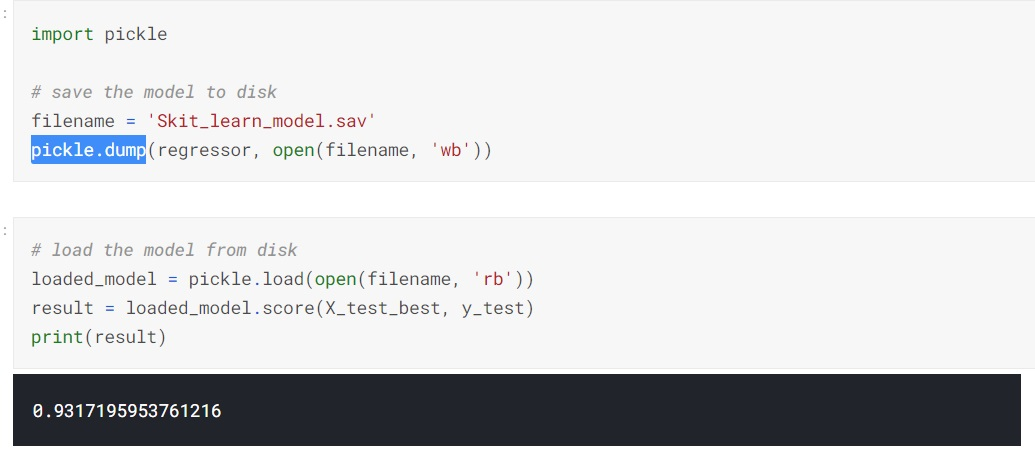
\includegraphics[width=0.8\columnwidth]{Pictures/scikitlearn_pickel.jpg}
	\caption[Short title]{Save and Load scikit learn model with pickle}
	\label{figure:scikitpickle}
\end{figure}

The model also can be trained with "GPU" to accelerate the training process and load with "CPU" later to save the memory.

In figure \ref{figure:savetorch} and \ref{figure:loadtorch} the model had been trained with GPU and later load in CPU using pytorch libraries. 

\begin{figure}[H]
	\centering
	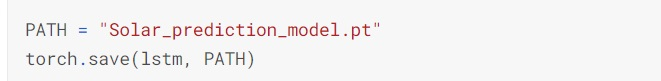
\includegraphics[width=0.8\columnwidth]{Pictures/save_LSTM.jpg}
	\caption[Short title]{Save Pytorch model}
	\label{figure:savetorch}
\end{figure}

\begin{figure}[H]
	\centering
	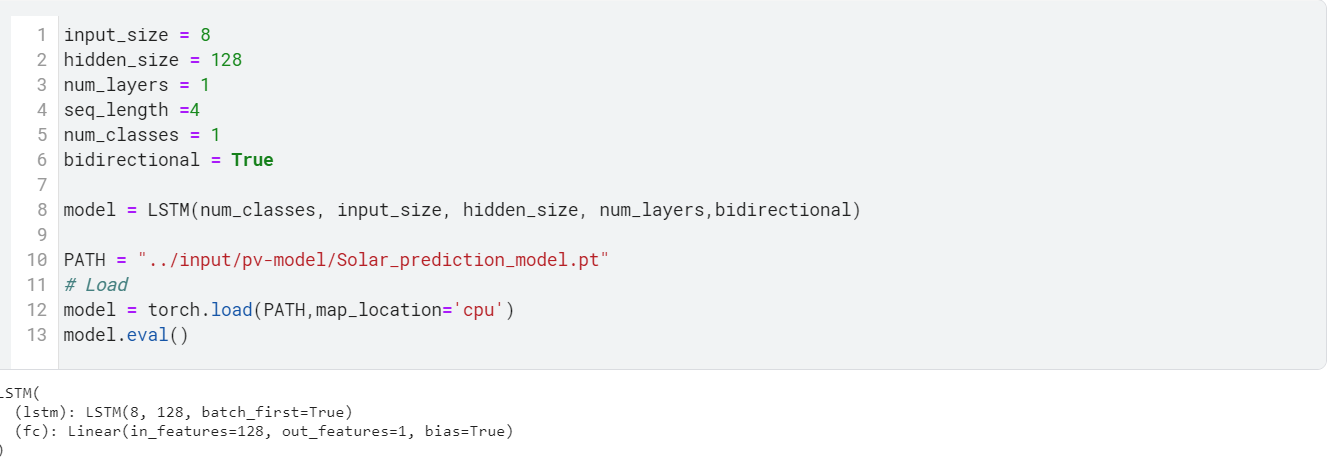
\includegraphics[width=0.8\columnwidth]{Pictures/load lstm.png}
	\caption[Short title]{Load Pytorch model}
	\label{figure:loadtorch}
\end{figure}

\newpage

\section{Model deployment}
\subsection{Deploy the model locally using Voila}

Voilà allows you to convert a Jupyter Notebook into an interactive dashboard that allows you to share your work with others. It is secure and customizable, giving you control over what your readers experience \cite{Voila}.

Install Voila with conda (figure \ref{figure:Voila}).

\begin{figure}[H]
	\centering
	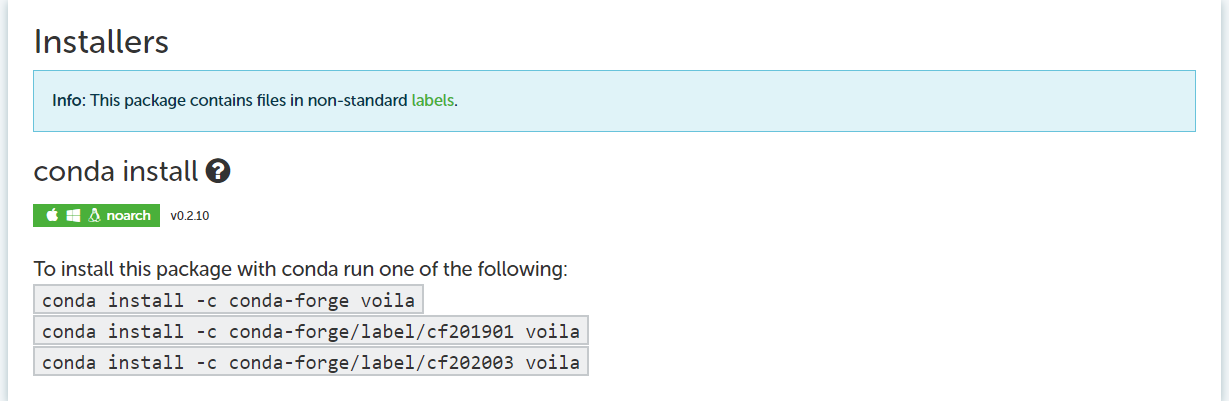
\includegraphics[width=0.8\columnwidth]{Pictures/Voila.png}
	\caption[Short title]{Voila package install}
	\label{figure:Voila}
\end{figure}

Move to the Jupiter notebook directory using cd "name of directory" and Run the Voila command : voila \textcolor{	red}{notebooknames}.ipynb. An example is shown in figure \ref{figure:Voila Run}.

\begin{figure}[H]
	\centering
	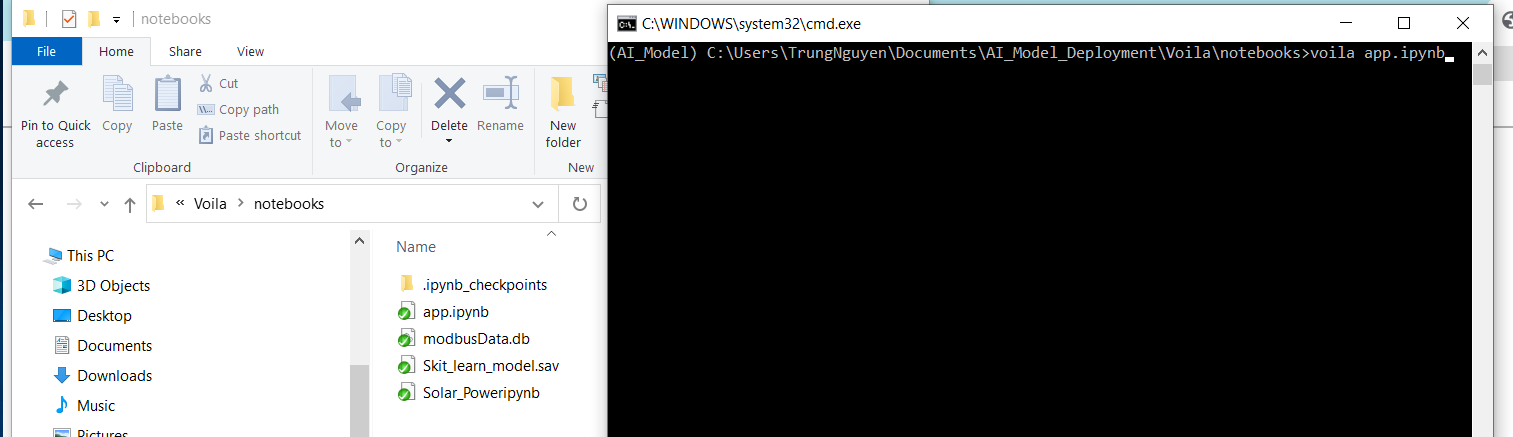
\includegraphics[width=0.8\columnwidth]{Pictures/Voila Run command.png}
	\caption[Short title]{Voila Run Command}
	\label{figure:Voila Run}
\end{figure}

A web browser with localhost address (figure \ref{figure:Voila Web}) will be 
opened 

\begin{figure}[H]
	\centering
    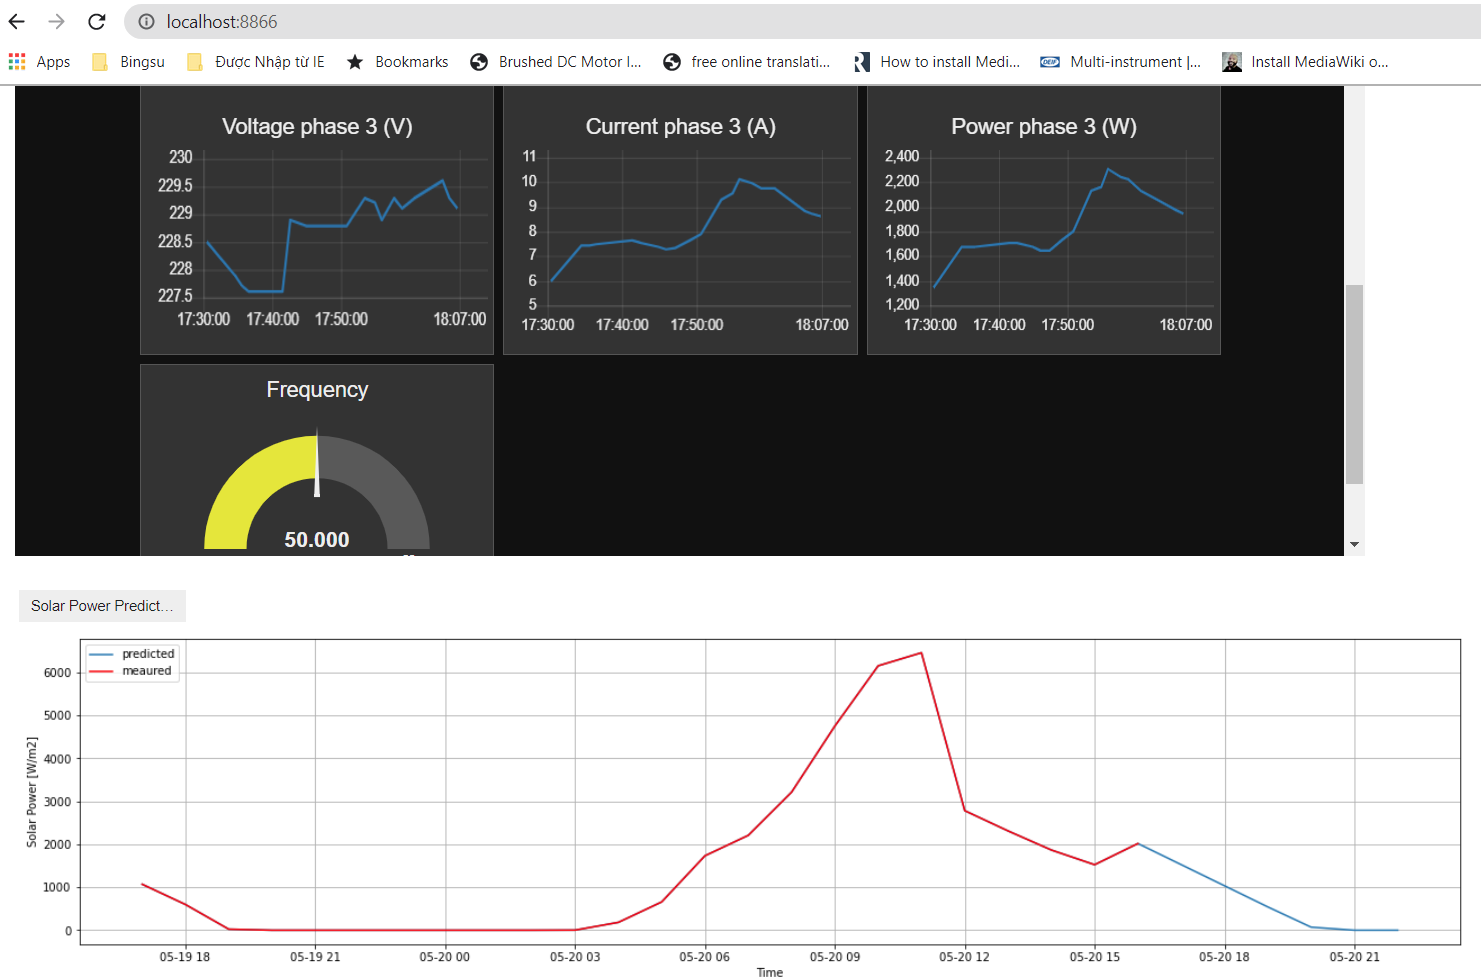
\includegraphics[width=0.8\columnwidth]{Pictures/Voila web example.png}
	\caption[Short title]{Voila Web}
	\label{figure:Voila Web}
\end{figure}

% https://voila.readthedocs.io/en/stable/deploy.html

\subsection{Deploy the model with Heroku}

Heroku is a cloud Platform that helps developers quickly deploy, manage, and scale moderns applications. Heroku provide a free package for non commercial app such as proof of concept and personal project \ref{figure:Heroku pricing}.

\begin{figure}[H]
	\centering
    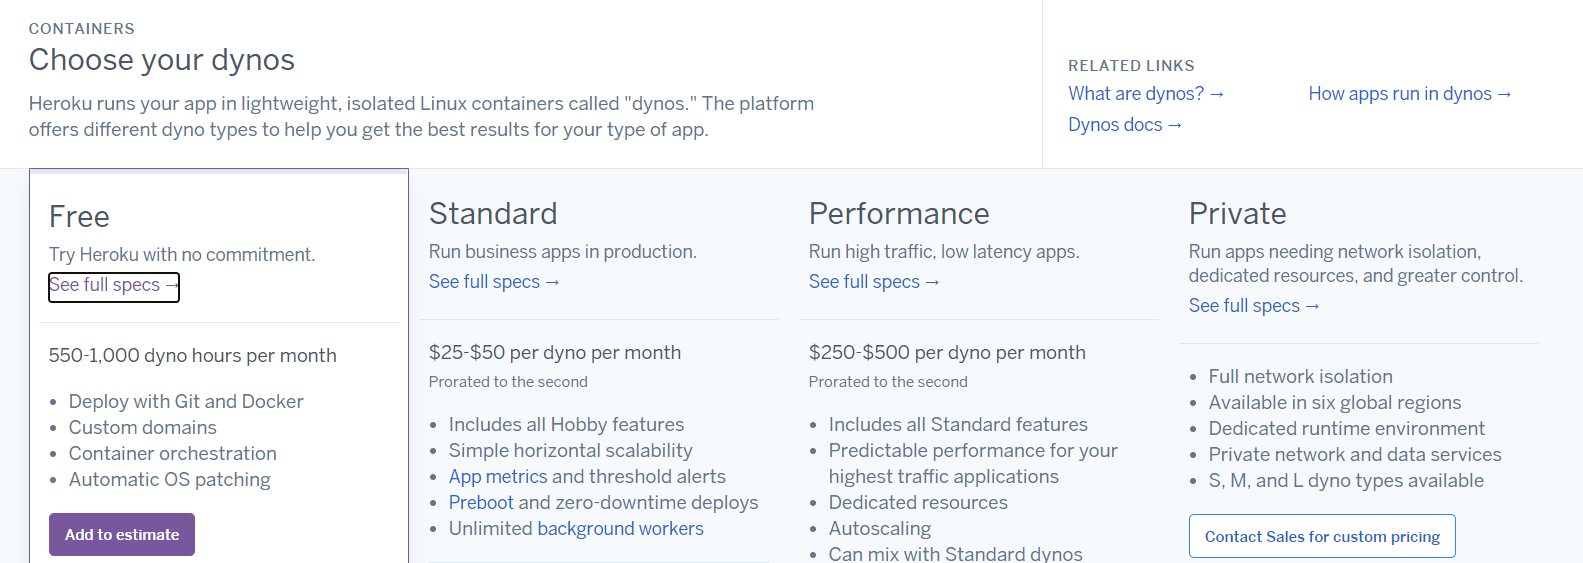
\includegraphics[width=0.8\columnwidth]{Pictures/Heroku packages.png}
	\caption[Short title]{Heroku Pricing}
	\label{figure:Heroku pricing}
\end{figure}

The first step is to create three files that Heroku requires.

\begin{itemize}
    \item requirements.txt : tells Heroku which Python packages to install when it run the web app.
    \item runtime.txt : specifies the version of Python we want Heroku to use.
    \item procfile: This file includes the instructions for Heroku to deploy our Voila app.
\end{itemize}

An example github prepare for Heroku deployment is shown on figure \ref{figure:Heroku github}. The notebooks folder content the jupyternotebook. 

\begin{figure}[H]
	\centering
    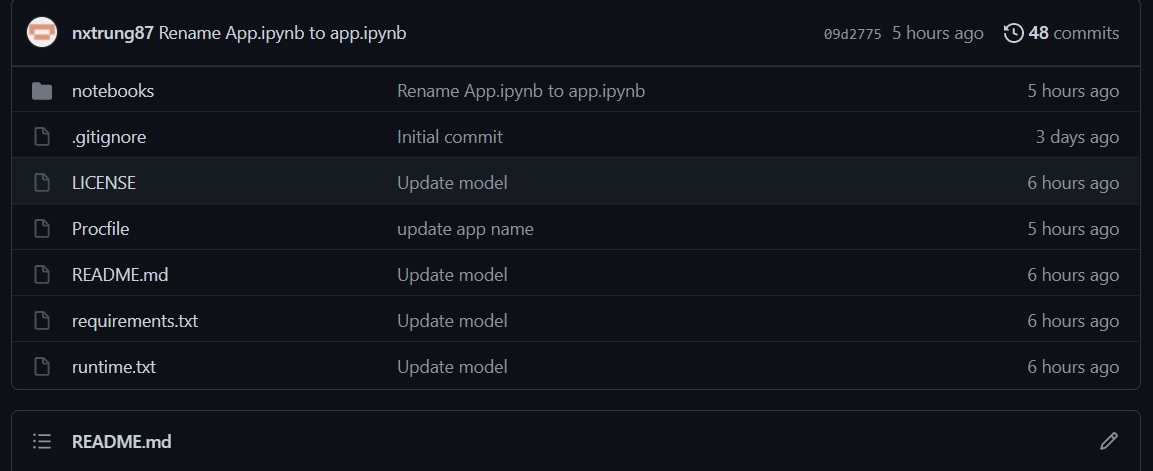
\includegraphics[width=0.8\columnwidth]{Pictures/Hroku_git.jpg}
	\caption[Short title]{Heroku github example}
	\label{figure:Heroku github}
\end{figure}

The contents example of the three Heroku require files is shown on figure \ref{figure:Heroku file content}. On the top left of the figure is the requirements.txt, top right is the runtuime.txt and bottom is the Procfile.

\begin{figure}[H]
	\centering
    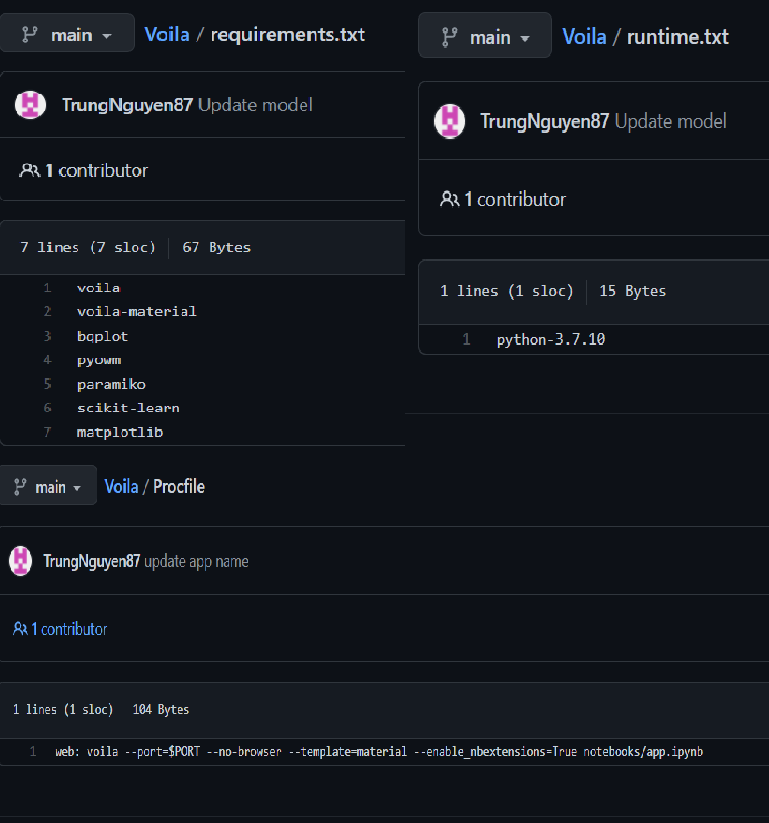
\includegraphics[width=0.8\columnwidth]{Pictures/Voila_heroku_files.png}
	\caption[Short title]{Heroku files content example}
	\label{figure:Heroku file content}
\end{figure}

\newpage

Next step is create an account with Heroku and follow the instruction in figure \ref{figure:Create new app}, \ref{figure:Create new app ctn}, \ref{figure:setup deployment}, \ref{figure:setup deployment method}, \ref{figure:web link}

In figure \ref{figure:Create new app} select new on the right corner.

\begin{figure}[H]
	\centering
    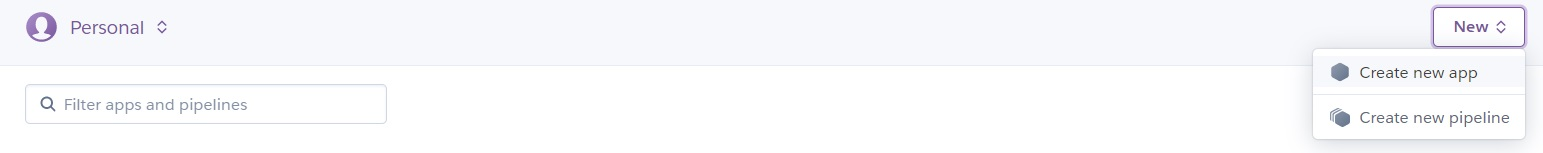
\includegraphics[width=0.8\columnwidth]{Pictures/Heroku_newapp.jpg}
	\caption[Short title]{Create new app}
	\label{figure:Create new app}
\end{figure}

Give a name for the app using lower letter case, select the deployment region and then select the create app button on the bottom.

\begin{figure}[H]
	\centering
    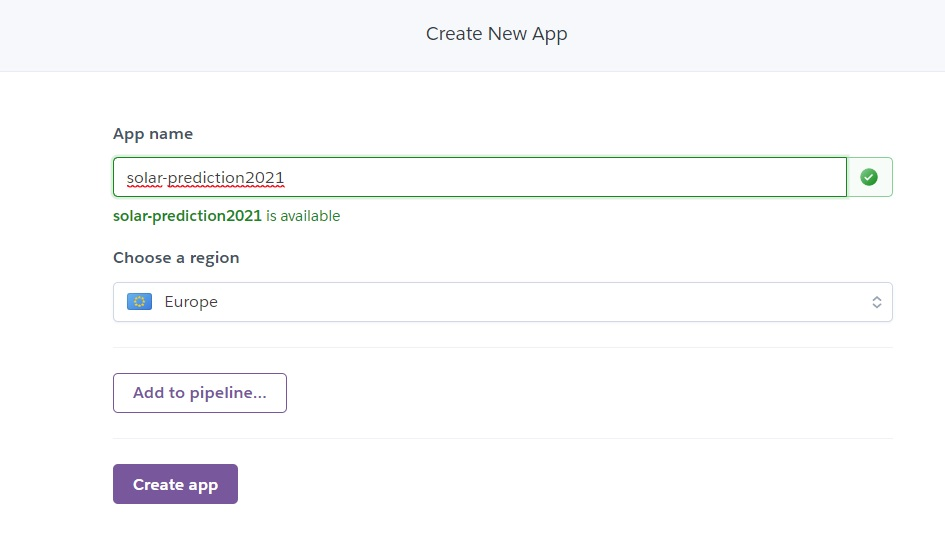
\includegraphics[width=0.8\columnwidth]{Pictures/Heroku_app.jpg}
	\caption[Short title]{Create new app ctn}
	\label{figure:Create new app ctn}
\end{figure}

In figure \ref{figure:setup deployment} select the Deploy tab and connect your app github repository. Scroll down and choose to enable the automatic deploys in figure \ref{figure:setup deployment method}.

Automatic deploys means every time when something is changed (for example update the requirement file or code file), the web app will also be updated. 

\begin{figure}[H]
	\centering
    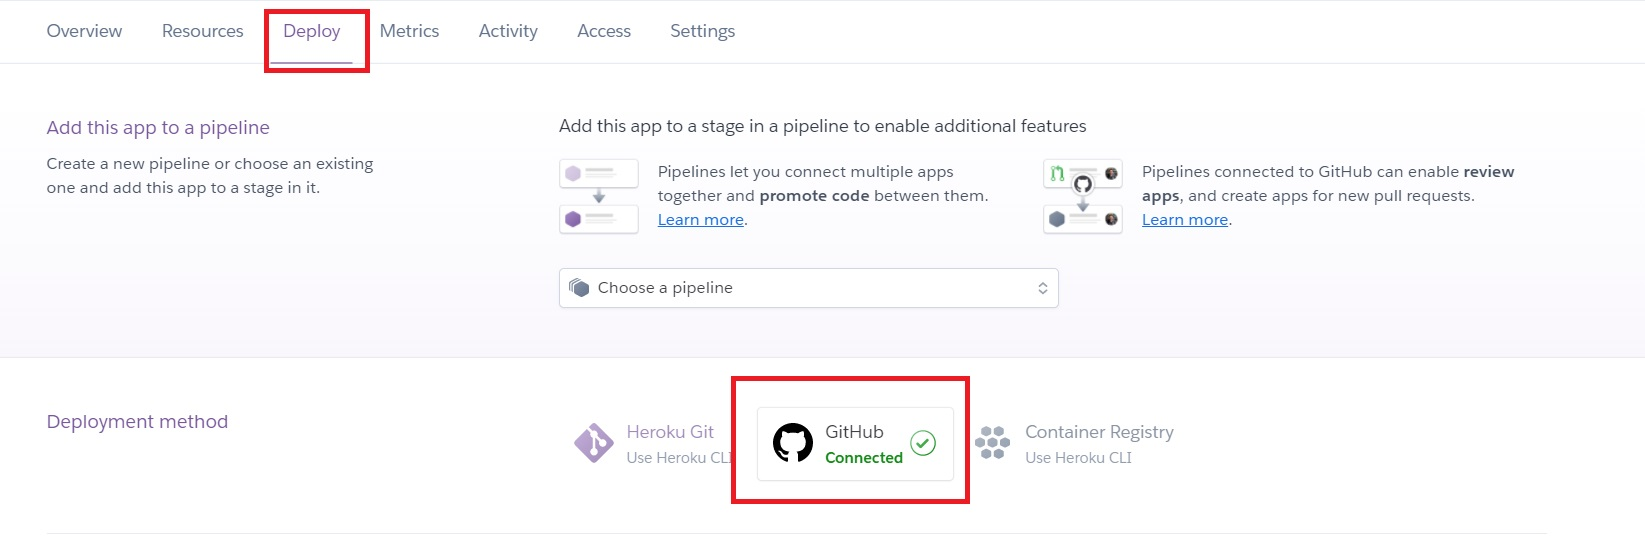
\includegraphics[width=0.8\columnwidth]{Pictures/Heroku_Deployment_setting.jpg}
	\caption[Short title]{Set up deployment}
	\label{figure:setup deployment}
\end{figure}

\begin{figure}[H]
	\centering
    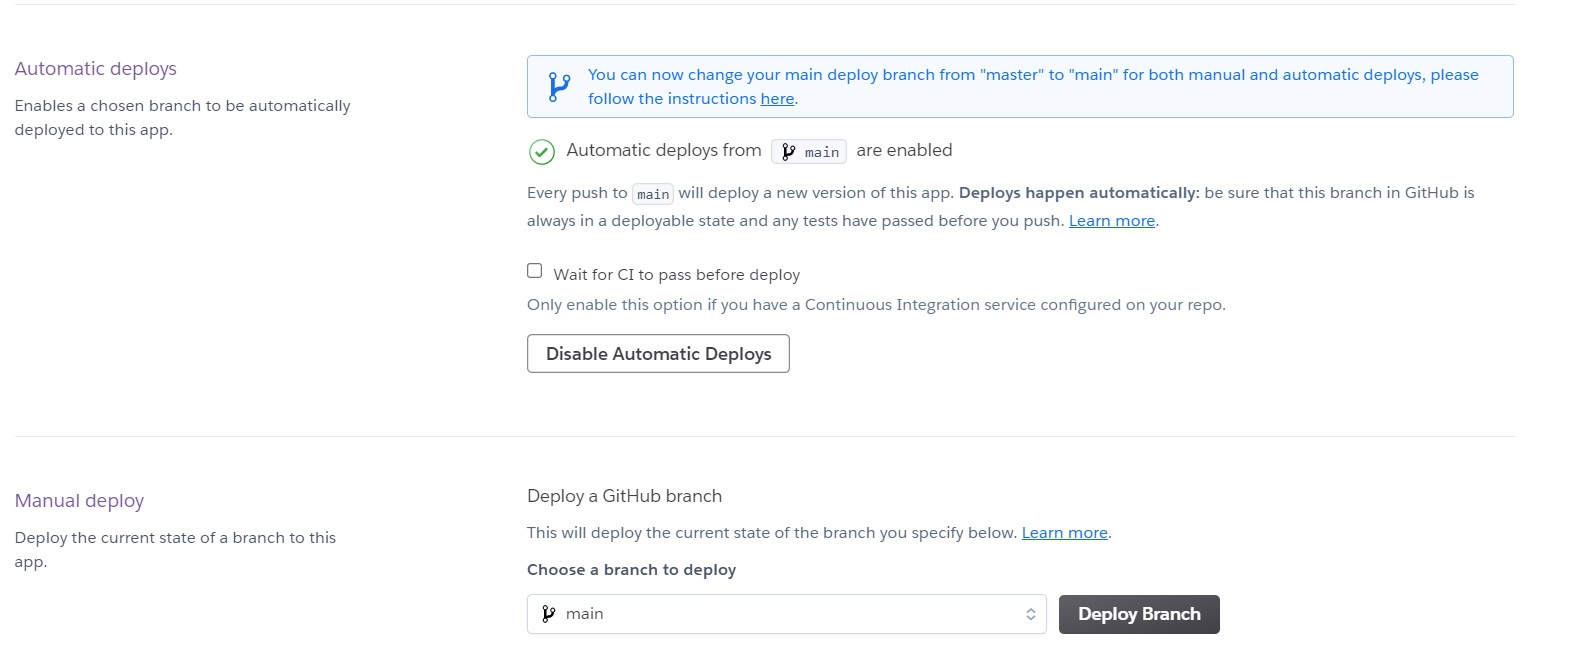
\includegraphics[width=0.8\columnwidth]{Pictures/Heroku_Deployment_methods.jpg}
	\caption[Short title]{Set up deployment method}
	\label{figure:setup deployment method}
\end{figure}

Link to the web app can be found on setting tab, scroll down to domains section (figure \ref{figure:web link}). User can also add their own domain name.

\begin{figure}[H]
	\centering
    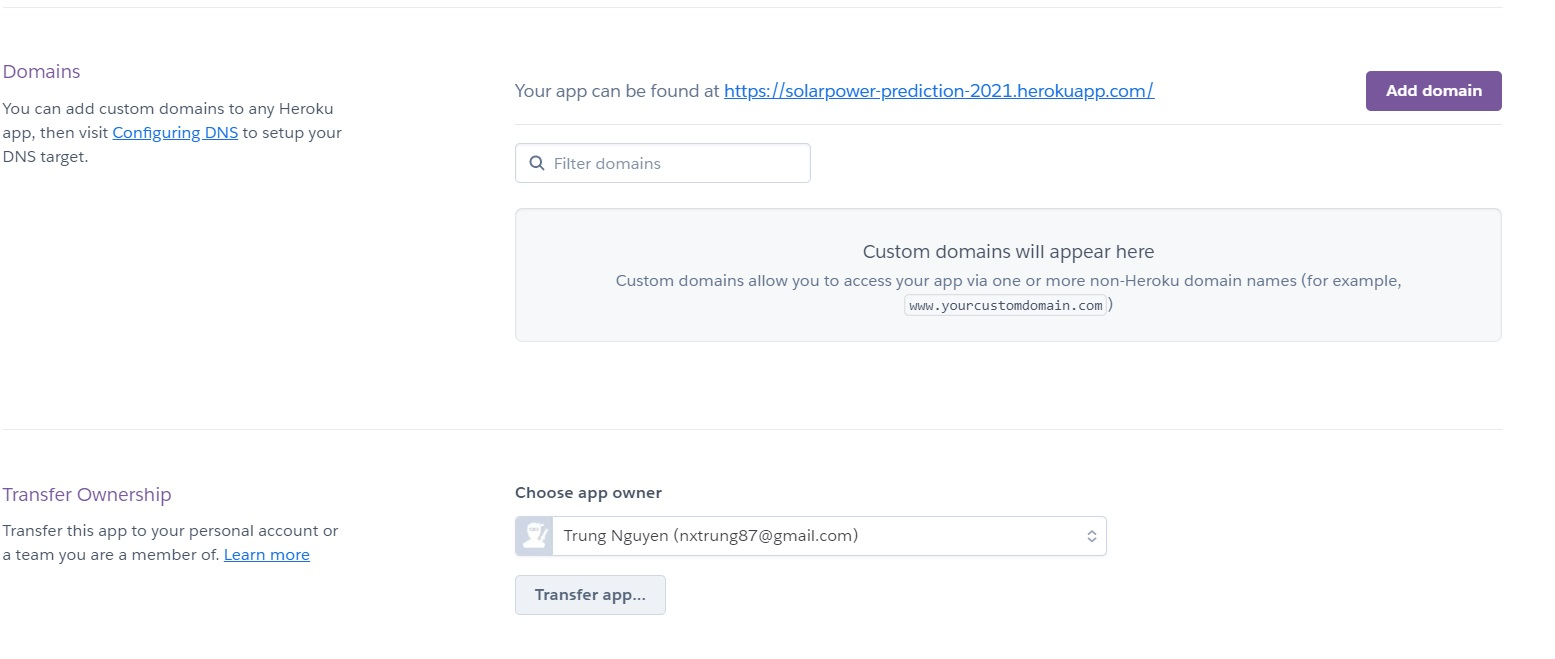
\includegraphics[width=0.8\columnwidth]{Pictures/Personal webapp.jpg}
	\caption[Short title]{Link of the web app}
	\label{figure:web link}
\end{figure}

Figure \ref{figure:web app} is a demo web app.

\begin{figure}[H]
	\centering
    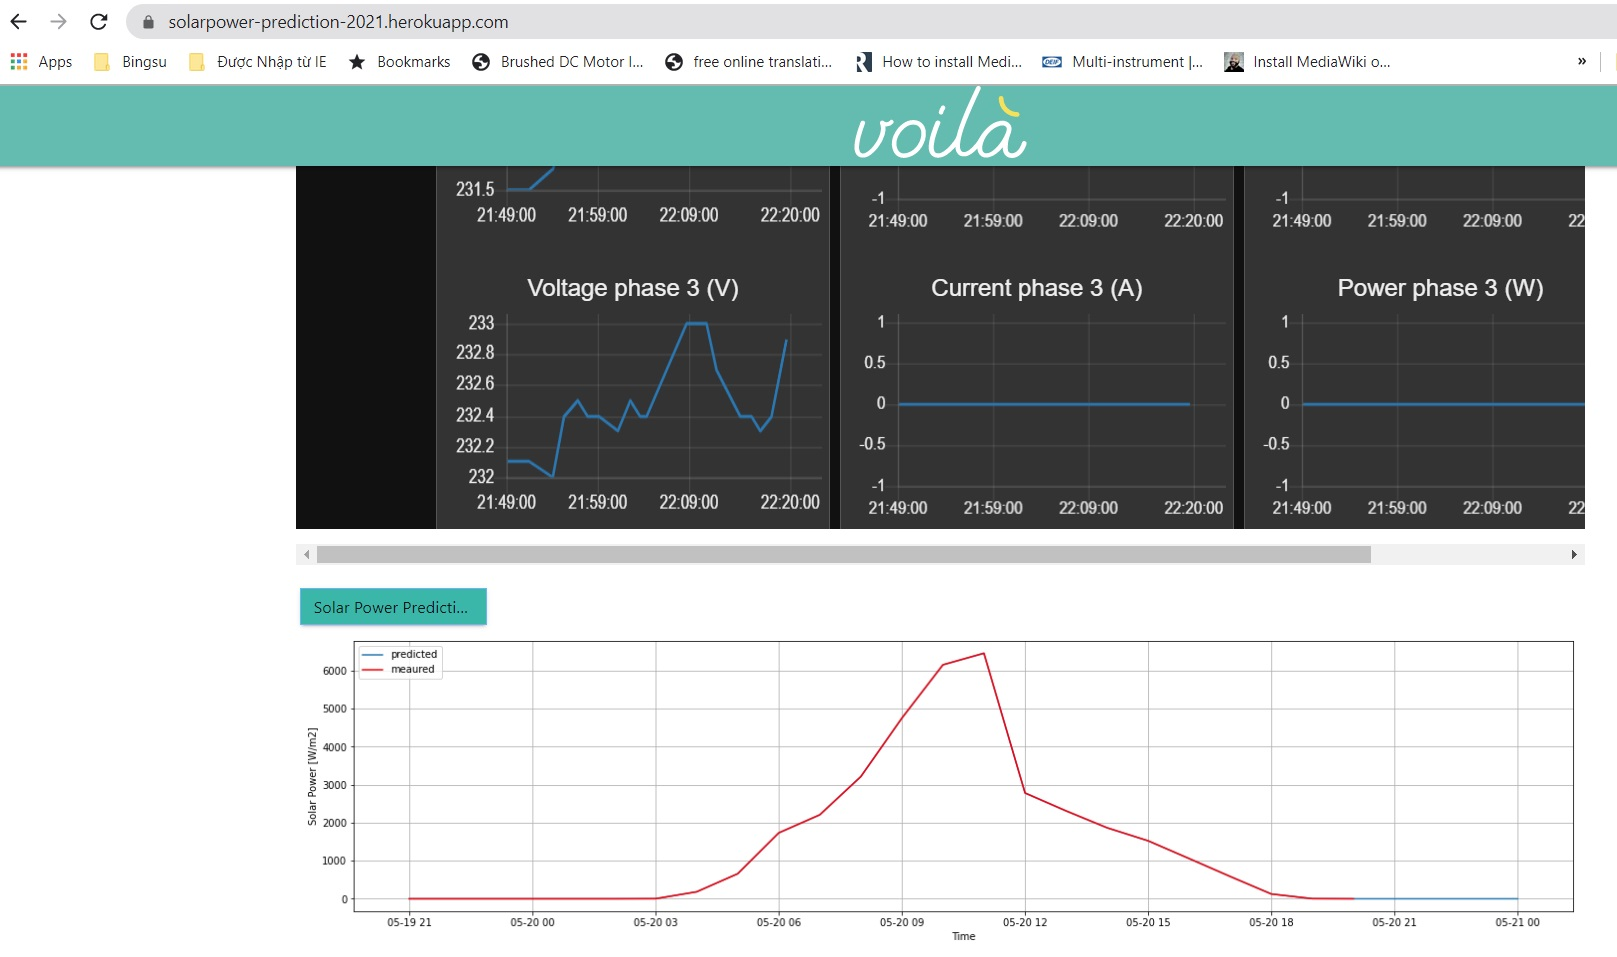
\includegraphics[width=0.8\columnwidth]{Pictures/Demo webapp.jpg}
	\caption[Short title]{The demo webapp}
	\label{figure:web app}
\end{figure}

\subsection{Forked the demo Github}

For the users who would like to try something quick. Forked the demo github repository (figure \ref{figure:Forked repo}) using the forked button on top right of the demo github page and follow the instruction to setup the deployment app with Heroku in the previous section.

\begin{figure}[H]
	\centering
    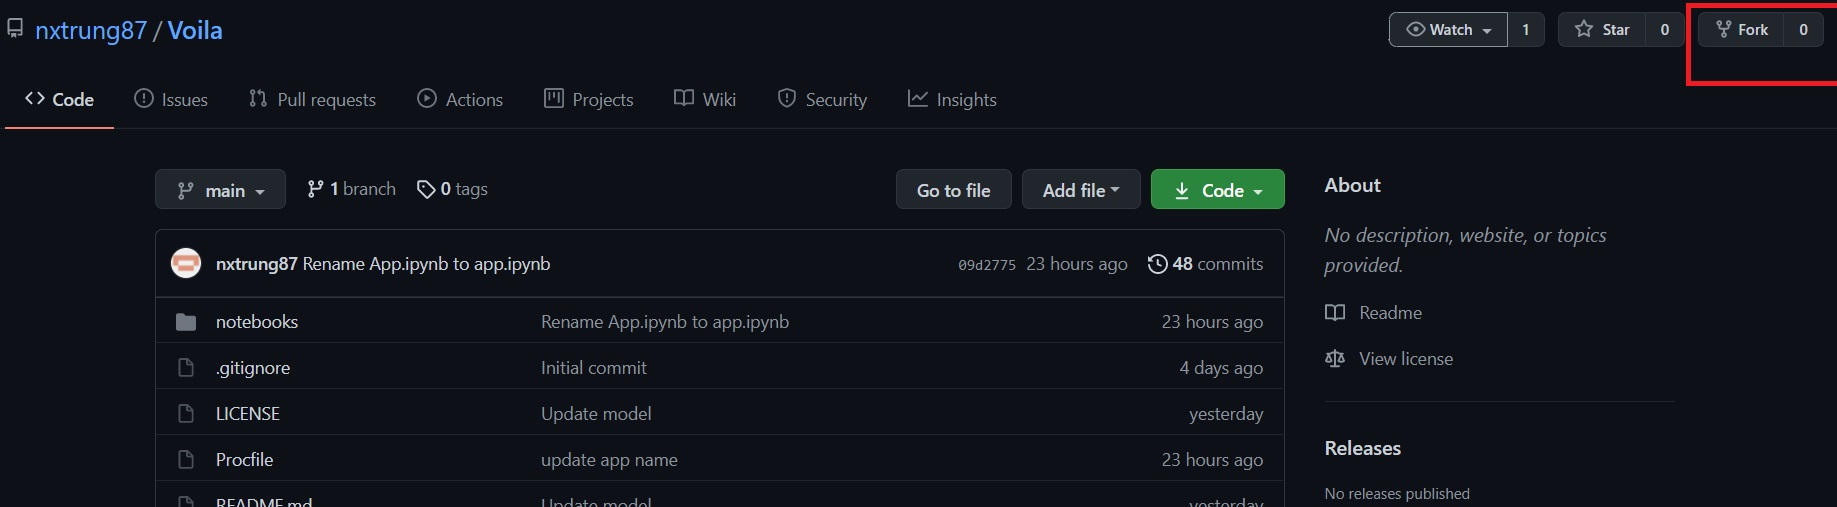
\includegraphics[width=0.8\columnwidth]{Pictures/forked repository.jpg}
	\caption[Short title]{Forked a repository}
	\label{figure:Forked repo}
\end{figure}

A few more demo github page to try out:
\begin{itemize}
    \item \hyperlink{https://github.com/voila-dashboards/voila-heroku}{voila-heroku}.
    \item \hyperlink{https://github.com/maartenbreddels/voila-demo}{voila-demo}.
    \item \hyperlink{https://github.com/jtpio/jupyterlab-heroku}{jupyterlab-heroku}.
\end{itemize}


\newpage


% \input{2R2Cmodel}

\section{Link to relevant information}

More information about online - offline deployment platform can be found on the links below.\newline

\begin{itemize}
	\item \href{https://towardsdatascience.com/10-ways-to-deploy-and-serve-ai-models-to-make-predictions-336527ef00b2}{10 Ways to Deploy and Serve AI Models to Make Predictions}
	\item \href{https://www.freecodecamp.org/news/deploy-your-machine-learning-models-for-free/}{7 ML Model Deployment Cloud Platforms}
	\item \href{https://voila.readthedocs.io/en/stable/deploy.html}{Deploying Voilà}
	

\end{itemize}

\newpage


% \input{7R4Cmodel}

% \section{NEN and ISO}

The list of NEN and ISO standard used in the calculation:

\begin{itemize}
    \item NTA 8800
    \item NEN 1068
    \item ISO 6946
    \item ISO 10077-2
    \item NEN 7120
\end{itemize}

\newpage


%\bibliography{mybibliography}
\printbibliography[heading=bibintoc]

\end{document}



